\documentclass[Bachelorarbeit.tex]{subfiles}
\begin{document}

\graphicspath{{./figures/interpretation/}}	%specifying the folder for the figures

\chapter{Interpretation}
\label{ch:interpretation}

In this chapter the interpretation of the results of chapter \ref{ch:results} are given and discussed where the central question is whether the Ascending-Connected topology satisfies the hypothesis or not. Thus only this topology is handled - both with and without importance sampling - because it is the most minimal network which satisfies the requirements for the hypothesis. The interpretations for the results of Hub-, Scale-Free and Small-World Topologies are handled in appendix \ref{app:results} but only to a minimal extent as they turn out to fall far from satisfying the hypothesis and the equilibrium because almost all of them do not meet the requirements but show interesting behaviour.

\section{Validating the Hypothesis}
When comparing the results of Ascending-Connected topology with and without importance sampling from Chapter \ref{ch:results} of figure \ref{fig:wealth_ASCENDINGCONNECTED_IS_100_NOCOLLATERALMARKET_REPL} and \ref{fig:wealth_ASCENDINGCONNECTED_100_NOCOLLATERALMARKET_REPL} with the results of the Fully-Connected topology of figure \ref{fig:wealth_FULLYCONNECTED_100_NOCOLLATERALMARKET_REPL} it becomes immediately clear that the equilibrium is different from the one of the Fully-Connected network and thus theoretical equilibrium is not reached in the case of Ascending-Connected topology neither with or without importance sampling. Although the visual results come quite close to the Fully-Connected one - there is a clear distinction between pessimists, medianists and optimists and the wealth-distribution looks about the same as in fully-connected - there remain serious artefacts in the range of the pessimists. Thus the property of the hypothesis is just necessary but not sufficient.

TODO HV: ist der Ausduck maximally short ein bekannter? mir scheint er in sich widerspruechlich
TODO HV: erklaere kurz wieso nicht

\section{Analysing artefacts}
Obviously the artefacts in the range of the pessimists indicate a miss-allocation of wealth, which are in fact collateralized assets. Pessimists, as noted in Chapter \ref{ch:leverageCycle}, are maximally short on assets and bonds and hold only cash, thus it is clearly a miss-allocation. As will be shown it comes from the fact that the pessimists want to sell but no neighbour is able to buy any more - a scenario which is not possible in Fully-Connected topology and is thus unique to Ascending-Connected networks with and without importance sampling.

\subsection{Dynamics of a single run}
\label{sub:dynamics_singlerun}
To better understand how such artefacts arise one needs to investigate the dynamics of a single run of the Ascending-Connected topology. The tools used are both the \textit{market-activity} and \textit{wealth-distribution} diagrams where the former one shows for each point of time the relative activity strength of each market. Being active means a successful match on a given market which implies that in a successful matching-round only one market can be active as only one match on a specific market happens during a successful matching round. Because of this a moving window of size 100 is used to create a moving-average filter over all active markets where the result is normalized and all market-activity sums to 1.0 at each point in time of the diagram. This allows for a very good visual analysis of distinct trading-stages because noise is reduced but the overall trend of a market can be still seen clearly.

\medskip

3 trading-stages can be identified in the market-activity diagram of Ascending-Connected topology.

\begin{figure}[H]
	\centering
  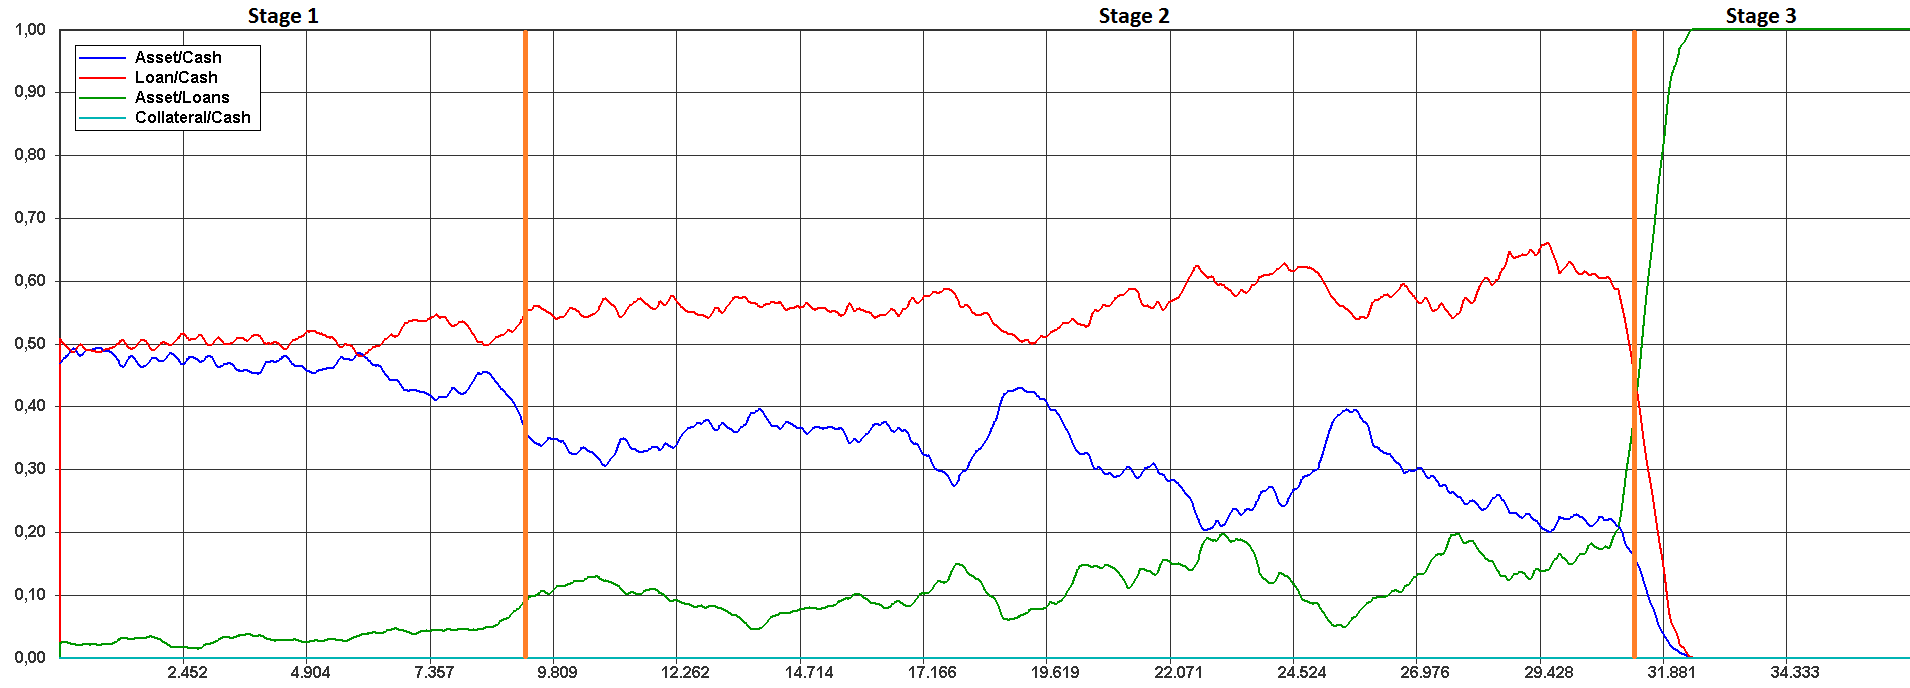
\includegraphics[width=1.0\textwidth, angle=0]{ASCENDINGCONNECTED_100_NOCOLLATERALMARKET_MARKET_STAGES.png}
  	\caption{Market-activity stages of Ascending-Connected topology}
	\label{fig:markets_ASCENDINGCONNECTED_100_NOCOLLATERALMARKET_MARKET_STAGES}
\end{figure}

TODO HV: collateral gegen cash gibt es hier doch gar nicht

\paragraph{Stage 1}
The allocations are very random overall but pessimists can be identified already as they sell their free assets against cash thus holding primarily cash but lots of collateralized assets are in the pessimists-range as well. Real distinction of optimists is not yet visible and medianists are far from showing up.

\medskip

The Asset/Cash and Bond/Cash markets are very dominant in this stage as the pessimists try to get cash for their free assets where the Asset/Bond market is hardly active but contributes enough to create the miss-allocation of the collateralized assets in the pessimists-range already.

\begin{figure}[H]
	\centering
  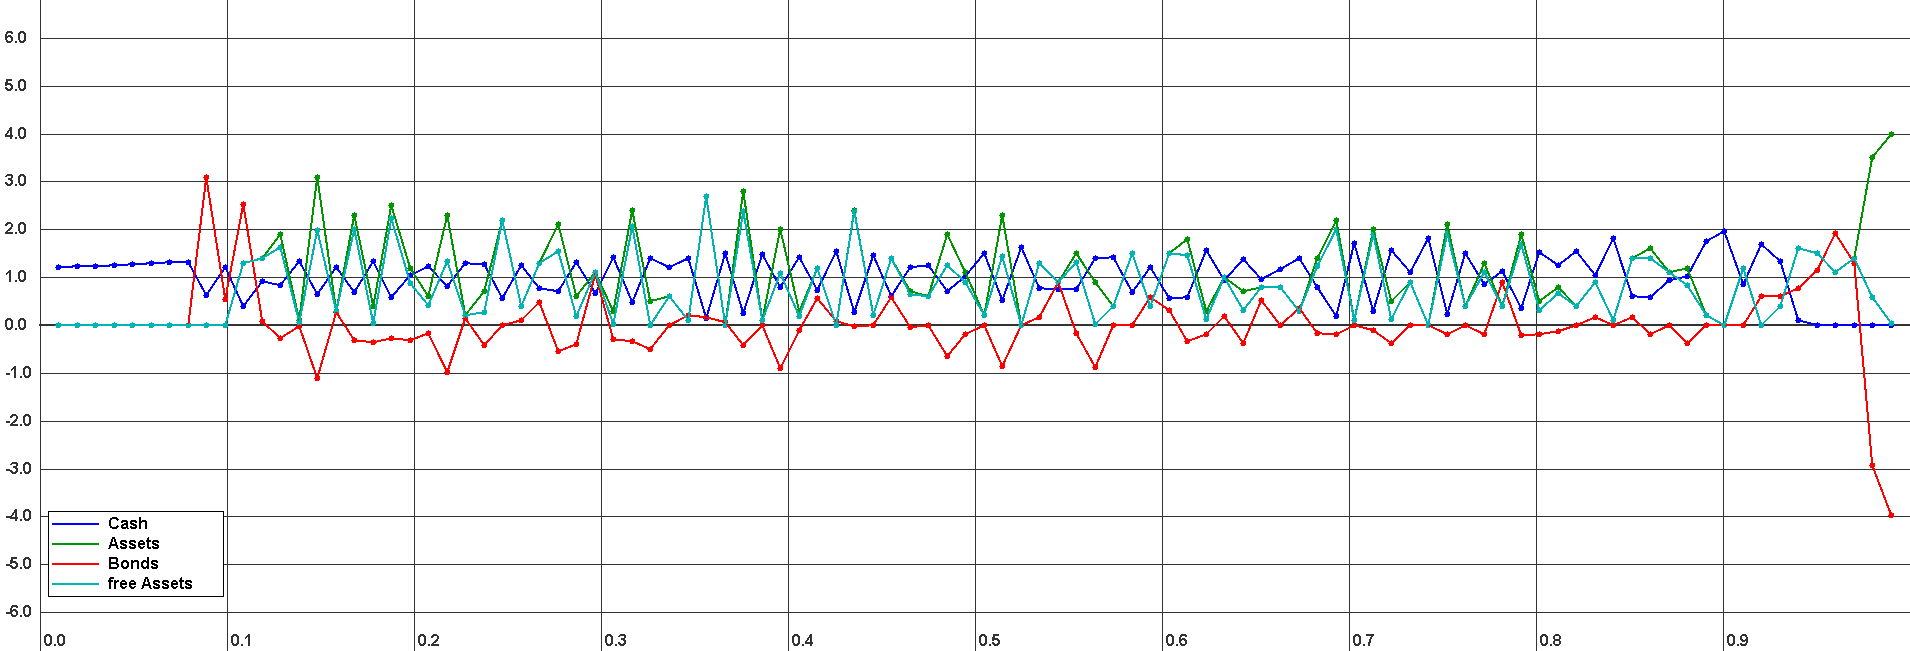
\includegraphics[width=1.0\textwidth, angle=0]{ASCENDINGCONNECTED_100_NOCOLLATERALMARKET_WEALTH_STAGE_1.png}
  	\caption{Wealth-Distribution of Ascending-Connected topology during Stage 1}
	\label{fig:markets_ASCENDINGCONNECTED_100_NOCOLLATERALMARKET_WEALTH_STAGE_1}
\end{figure}

TODO HV: es fehlt die Beschreibung, wie dieser Plot zustande kommt

\paragraph{Stage 2}
The pessimists which hold collateralized assets try to trade them up to the optimists which looks like waves when visualisizing it in the thesis-software. The optimists are now about to emerge as most of them are maximally short on cash and hold either free or collateralized assets. The medianists are still not visible yet.

TODO HV: ist die Vermoegensverteilung unten gemeint? da wuerde es nicht sinnvoll sein, von Wellen zu sprechen. Die Pessimisten kann man hier uebrigens besser charakterisieren. Naemlich so wie in Phase 3.

\medskip
		
The Asset/Cash market seems to go down in the long term while the Bond/Cash and Asset/Bond markets seems to increase. This is because fewer and fewer assets can be traded against cash because the optimists are already very low on cash thus the Asset/Bond market is naturally increasing as they can trade only on this market any more.
		
\begin{figure}[H]
	\centering
  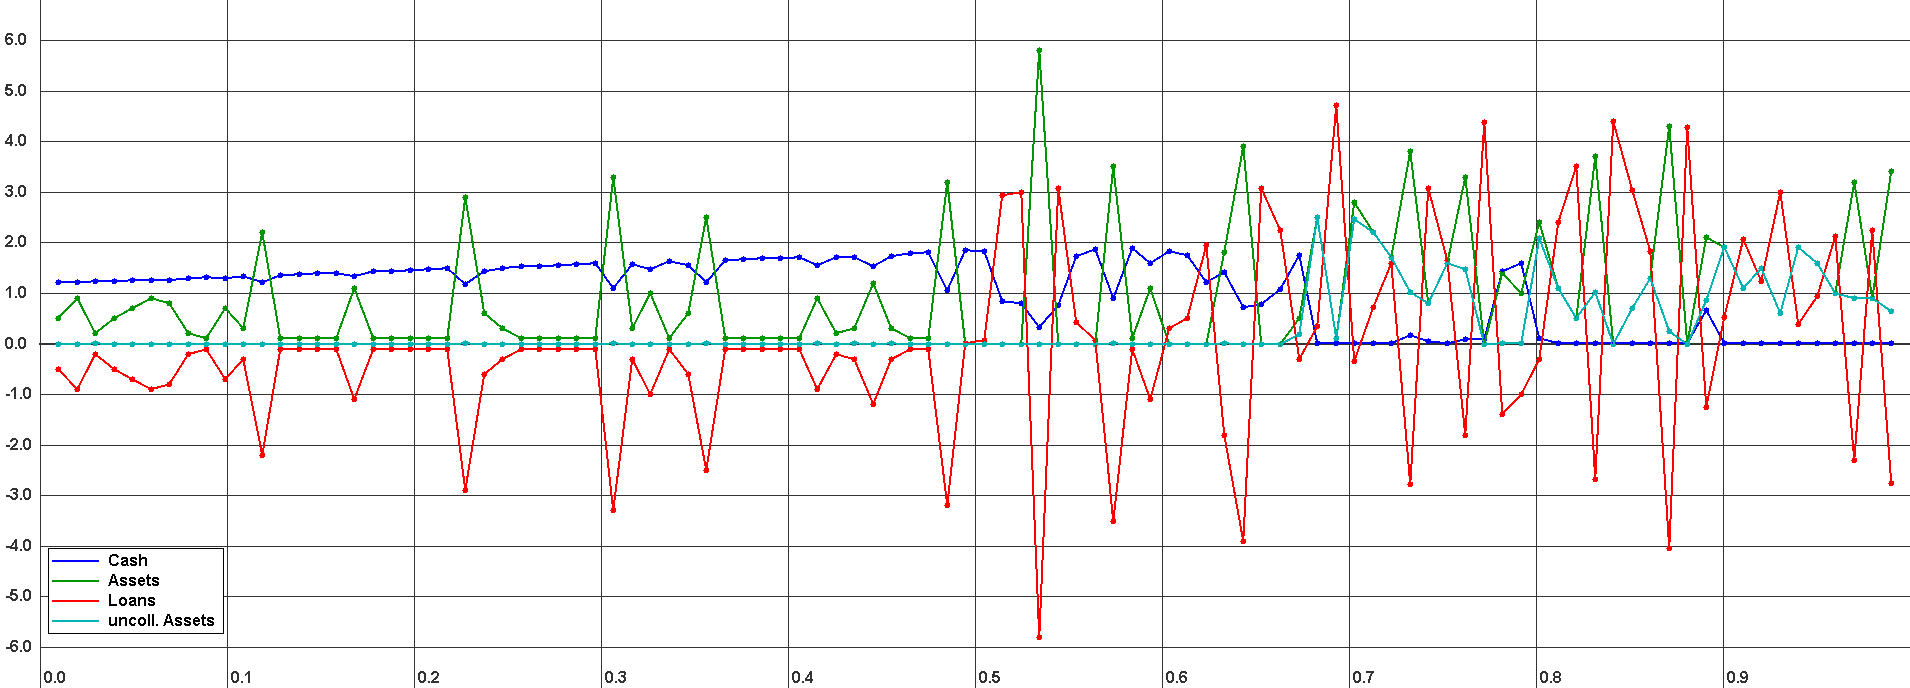
\includegraphics[width=1.0\textwidth, angle=0]{ASCENDINGCONNECTED_100_NOCOLLATERALMARKET_WEALTH_STAGE_2.png}
  	\caption{Wealth-Distribution of Ascending-Connected topology during Stage 2}
	\label{fig:markets_ASCENDINGCONNECTED_100_NOCOLLATERALMARKET_WEALTH_STAGE_2}
\end{figure}
		
\paragraph{Stage 3}
The pessimists lie dormant and are completely inactive. The medianists begin to show up holding only bonds and the real optimists begin to crystallize holding only collateralized assets. These two frontiers move towards each other as only collateralized assets can be traded any more as both medianists and optimists hold only collateralized assets and bonds. TODO HV: stimmt nicht nach dem plot

\medskip

The Asset/Cash market lies dormant because the pessimists are no more able to trade and the optimists are maximally low on cash. The Bond/Cash market is inactive too whereas the Asset/Bond market takes over and dominates 100\% as only collateralized assets are traded any more as stated above.

TODO HV: why not?? hier ist die Beschreibung viel zu geheimnisvoll
TODO HV: falsch - dafuer gibt es hier gar keinen Markt! (Asset/Bond war damit gemeint)

\begin{figure}[H]
	\centering
  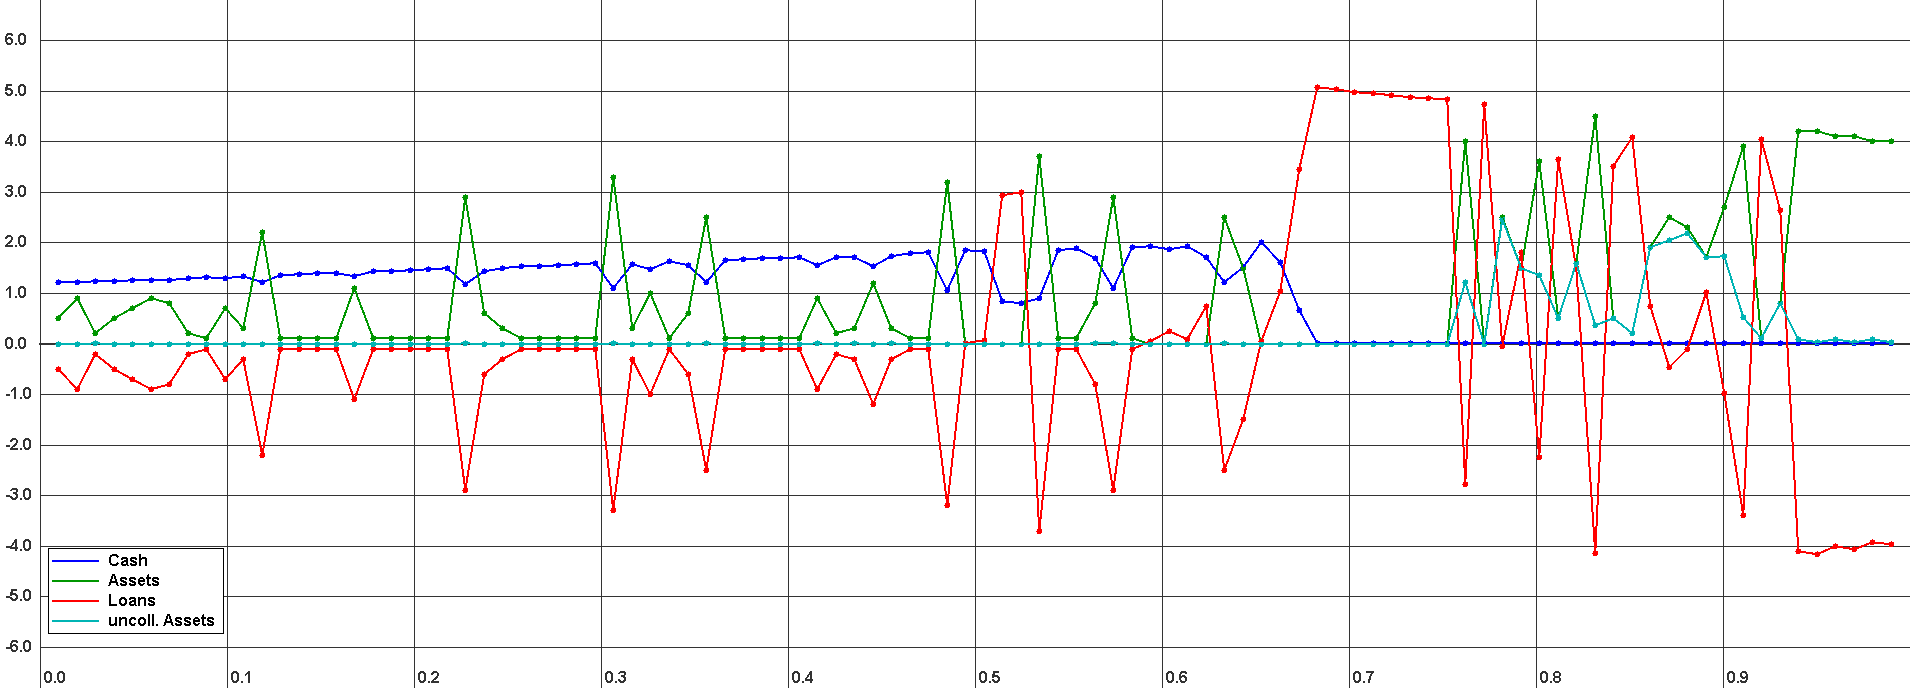
\includegraphics[width=1.0\textwidth, angle=0]{ASCENDINGCONNECTED_100_NOCOLLATERALMARKET_WEALTH_STAGE_3.png}
  	\caption{Wealth-Distribution of Ascending-Connected topology during Stage 3}
	\label{fig:markets_ASCENDINGCONNECTED_100_NOCOLLATERALMARKET_WEALTH_STAGE_3}
\end{figure}

\paragraph{Deriving the emerging of the artefacts}
TODO HV: zu lange und umstaendliche Erklaerung., ausserdem fehlt formale Beschreibung der Artefakte, alles ist viel zu intuitiv. Erst formal mit Formeln, dann ein paar Worte - siehe als Verbesserungsweg meinen Kommentar weiter unten.


The wealth stabilizes from both the left and the right end of the optimism-scale towards the i2-point where medianists become optimists - around this point the last trades will happen.

\medskip 

Pessimists try to sell all their assets against cash to the neighbour with higher optimism-factor.

\medskip 

Optimists try to buy as much assets as they can get from the neighbour with lower optimism-factor. In the beginning they use cash and after they've run out of cash they buy assets against bonds.

\medskip 

The medianists serve as connection between the pessimists and optimists transferring the assets to the optimists by buying from agents with lower optimism and selling to higher ones either through asset against cash or asset against bond.

\medskip 

Thus the assets move from the pessimists through the ascending chain of optimism to the optimists as no direct connection between these two groups exists with the medianists in between. Thus waves of uncollateralized assets can be seen moving from pessimists to optimists.

TODO HV: wo?? der Leser sieht hier keine Wellen!

\medskip 

It is important to understand that all agents independent of their optimism factor make offers on all markets if they are able to and their cash, collateral or bond constraints are satisfied. This implies that pessimists trade bonds as well as assets against bonds although they turn out to be pessimists. Note that the agents are not defined exogenous as pessimists/medianist/optimists but this property emerges during the simulation.

\medskip 

Thus pessimists gain wealth in collateralized assets too which can be seen by the green spikes with the same amount of negative bonds as those assets are bought against bond. Of course they try to sell it to neighbours with higher optimism factor but this is only possible if these neighbours are able to buy which they can only if they hold enough positive bonds to buy the offered asset for the offered amount of bonds.

TODO HV: zu ungenaue Beschreibung. Erklaere es mit Buchstaben fuer Preise und Mengen, und mit Ungleichungen auf diesen, welche Nebenbedingungen und positiven Utility Gewinn ausdruecken. Anschliessend kannst Du wieder versuchen, das Ganze in Woerter zu fassen - es ist nicht so leicht!

\medskip 

Whether an agent has enough wealth to buy from a seller is more or less random and depends on its trading history. Matching happens randomly and thus it is possible that the neighbourhood of a seller "dries up" as the potential buyers sold all their goods to the next agent with higher optimism factor and become thus unable to buy from the potential seller because they have no more positive bonds to buy assets against bonds. In such a case a potential pessimist seller of collateralized assets is then cut from its environment and becomes unable to trade any more resulting in a miss-allocation in collateralized assets.

\medskip 

It is also possible for a group of agents to get cut from its environment through this random trading-process. In this case the agents within this "island" still trade between each other resulting in the uncollateralizing of assets which immediately are traded towards optimists but as soon as a point is reached where no buyer is available with enough positive bonds to buy collateralized assets this island is also incapable of trading any more resulting in an island of miss-allocated wealth.

\medskip 

An important fact to notice is that the artefacts must not necessarily show up. It is possible for a single run to finish without these artefacts showing up. This is due to the random-process of sweeping and matching and thus the artefacts are subject to this random process too as noted in section \ref{sec:implementation_performanceImprovement}. Importance sampling elevates this problem a bit as it allows for more trades as the matching probabilities are very much increased but fails in the end for the same reason as the simulation without it - the artefacts are just "smaller" but show up almost always.

TODO HV: diese Technik kann hier ueberhaupt nicht helfen

\begin{figure}[H]
	\centering
  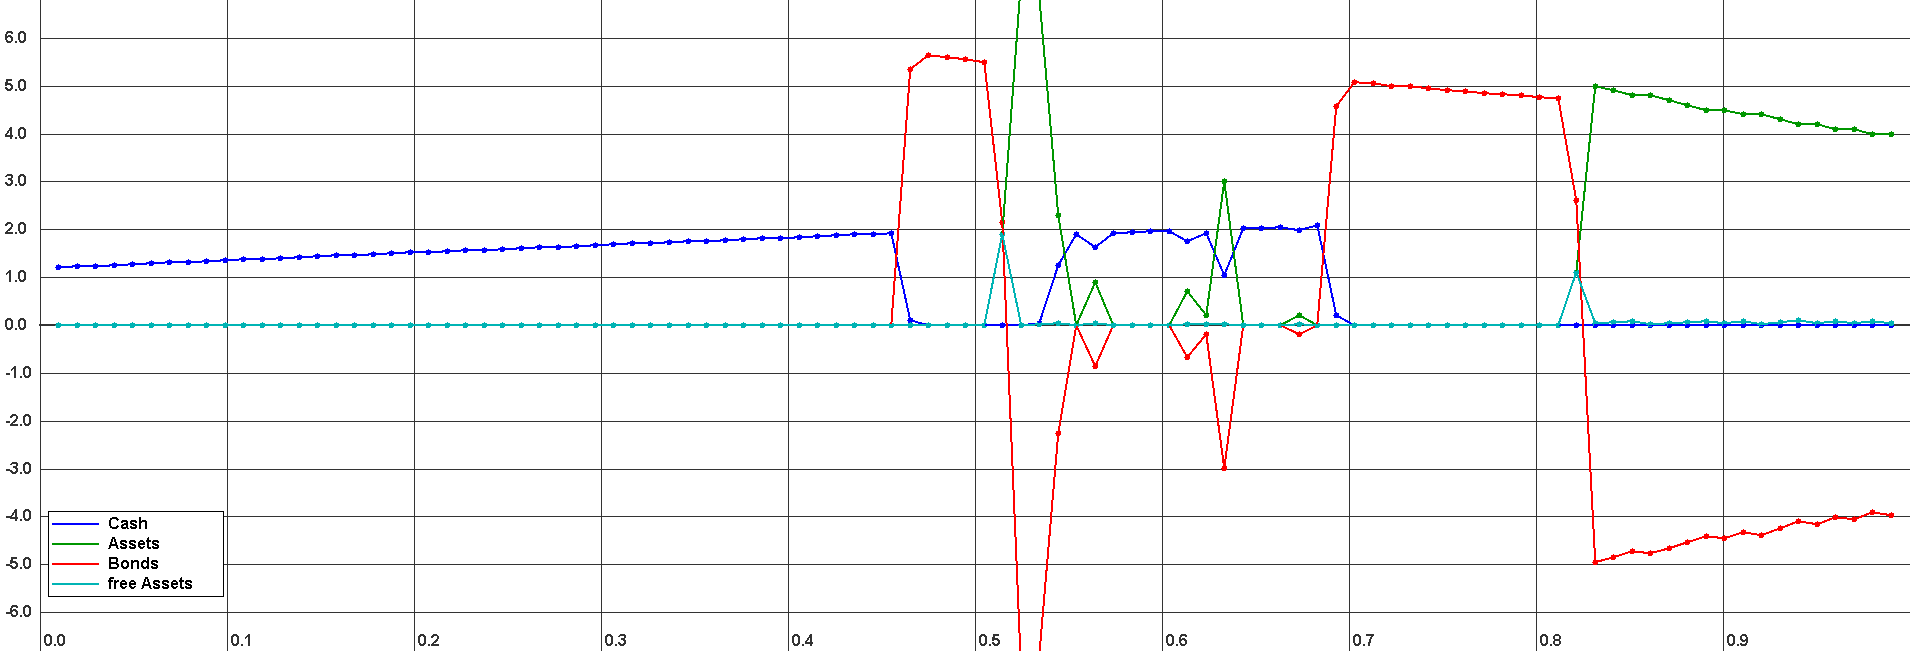
\includegraphics[width=1.0\textwidth, angle=0]{ASCENDINGCONNECTED_100_NOCOLLATERALMARKET_SINGLE.png}
	\caption{Final wealth-distribution of Ascending-Connected topology after a single run}
	\label{fig:wealth_ASCENDINGCONNECTED_IS_100_NOCOLLATERALMARKET_SINGLE}
\end{figure}

\section{Extending the Hypothesis}
After it has become clear that the hypothesis is wrong the question arises what needs to be done to correct it. It is clear that a mechanism needs to be found which prevents or resolves the arising of the artefacts within the pessimist wealth-range. Obviously two solutions are available.

\subsection{Approaching fully connectedness}
Increasing the connectedness of the topology increases the probability of global-optimal trades and allows more agents to trade between each other and thus the probability of resolving islands or artefacts of wealth miss-allocation is increased with the density of connectedness. TODO HV: wieso??
The experiments of ascending-connected topology with short-cuts were desigend to develop an understanding how the simulation behaves with increasing connectedness and also how the two types of  fully- and regular-connectedness influence the results.
It seems that full short-cuts seem to help dramatically in reducing the miss-allocations where the number of full short-cuts seems to be dependent on the number of agents which this thesis leaves for further research. See section \ref{app:results_acShortCuts} for a short overview of the results and interpretation of short-cut based Ascending-Connected topologies.
\linebreak
Of course in real environments approaching fully connectedness is not always possible and thus only the other mechanism is left as an option to resolve the artefacts.

\subsection{Re-Enabling trading}
\label{ch:interpretation_reenablingTrading}
Another way to look at the arising of the artefacts is in identifying them as suboptimal trades. \cite{Breuer2015} were confronted with this circumstance when they introduced the Asset/Bond Market where they found that the equilibrium was fundamentally different from the theoretical one because agents were trapped in suboptimal trades and couldn't reverse their decisions made earlier. The trades where suboptimal because each agent assigns depending on its optimism factor a different bond-value to each asset. As a solution they introduced the "Bonds-Pledgeability" (BP) mechanism which allows to trade bonds in both ways instead of only gathering them and not being able to sell them - see chapter \ref{ch:leverageCycle} for a more in-depth discussion of the BP-Mechanism.

\medskip 

Thus if those artifacts are treated as suboptimal trades one needs to introduce a mechanism similar to BP to allow the reversibility of suboptimal trades in the context of collateralized assets. The only possibility without altering the network-topology is to re-enable the pessimists to trade their collateralized assets against cash as all pessimists hold cash and are thus able to buy and sell collateralized assets against cash. This new mechanism is expected to repair the miss-allocated wealth and to restore the validity of the previously disproved hypothesis.

TODO HV: eigentlich hat das weder mit suboptimalen Handelsentscheidungen noch mit Reversibilitaet zu tun, sondern schlicht mit einer spezifischen Blockadesituation

\medskip 

See Chapter \ref{ch:newMarket} for the implementation and results of this new mechanism.

\end{document}
